% Chapter 5

\chapter{Analytical and Experimental Results} % Main chapter title

\label{Chapter5} % For referencing the chapter elsewhere, use \ref{Chapter1} 

\lhead{Chapter 5. \emph{Analysis and Conclusion}} % This is for the header on each page - perhaps a shortened title

%----------------------------------------------------------------------------------------
\section{Fourier Analysis}
\label{fourier}
One of the most pressing concerns regarding switching power supplies is the spectral content of the output signal, both before and after filtering. This is of chief concern to power systems designers because the demands that excess spectral content can place on filtering increase size, weight, and cost of the inverter system. These additional frequencies represent energy that must be dissipated by the filter, and hence an inefficiency in our system. A comparative analysis of the dominant PWM techniques is necessary to understand the costs and benefits of each technique, but more importantly for the purpose of this paper, to understand how the hybrid algorithm used to modulate pulse-widths stacks up. In this section we lean heavily on the work of Zhous in \cite{fourierAnalysis}. We contribute to this discussion by analyzing the performance of closed loop control, where Zhou strictly examines open loop PWM inverters.

Recall that any signal can be decomposed into a sum of sines and cosines given by the expression:
\begin{equation}
f_N(\omega t) = \frac{a_0}{2} + \sum_{n=1}^N \left(\overbrace{a_n}^{A_n \sin(\phi_n)} \cos(n\omega t) + \overbrace{b_n}^{A_n \cos(\phi_n)} \sin(n\omega t)\right)\\
= \sum_{n=-N}^N c_n\cdot e^{in\omega t}
\end{equation}

Where
\begin{align*}
& ~~~~~ a_0 = \frac{1}{T}\int_{0}^{T}f(t)dt \\
a_n &= \frac{2}{T}\int_{t_0}^{t_0+T} f(t)\cdot  \cos(n\omega t)\ dt \\
b_n &= \frac{2}{T}\int_{t_0}^{t_0+T} f(t)\cdot  \sin(n\omega t)\ dt \\
c_n &= \frac{1}{T}\int_{t_0}^{t_0+T} f(t)\cdot e^{-in\omega t}\ dt
\end{align*}

\begin{equation}
c_n \ \stackrel{\mathrm{def}}{=} \ \begin{cases}
\frac{A_n}{2i} e^{i\phi_n} = \frac{1}{2}(a_n - i b_n) & \text{for } n > 0 \\
\frac{1}{2}a_0 & \text{for }n = 0\\
c_{|n|}^*  & \text{for } n < 0.
\end{cases}
\end{equation}


The magnitude of every harmonic of the fundamental can be found by:

\begin{align*}
K_0 &= \frac{a_0}{2} \\
K_n &= \sqrt{a_n^2+b_n^2}
\end{align*}

Note that in all cases it is understood that $n\in \mathbb{Z}$.

Additionally, because direct application of the Fourier analysis can be cumbersome, the analysis of less friendly waveforms can be simplified by the application of the following properties of symmetry.

For \textbf{odd symmetry}, that is, functions satisfying the equality $f(t)=-f(-t)$ it is given that:
\begin{equation}
\begin{cases}
a_n = 0 \\ 
b_n = \frac{2}{\pi}\int_{0}^{\pi}f(\omega t)\sin(n\omega t)d\omega t
\end{cases}
\end{equation}

For \textbf{half-wave symmetry}:
\begin{equation} 
\begin{cases} 
C_n = 0 &\mbox{for even n}  \\ 
a_n = \frac{2}{\pi}\int_{0}^{\pi}f(\omega t)\cos(n\omega t)d\omega t &\mbox{for odd n}  \\
b_n = \frac{2}{\pi}\int_{0}^{\pi}f(\omega t)\sin(n\omega t)d\omega t &\mbox{for odd n} 
\end{cases}
\end{equation}

This condition holds when $f{\omega t} = -f(-\omega t + \frac{T}{2})$.

And for \textbf{quarter-wave symmetry}:
\begin{equation} 
\begin{cases} 
a_0 = 0 \\
a_n = 0 &\mbox{for even n}  \\
a_n = \frac{8}{T}\int_{0}^{\frac{T}{4}}\cos{n\omega t} &\mbox{for odd n}  \\
b_n = 0 &\mbox{for all n} 
\end{cases}
\end{equation}
Quarter-wave symmetry holds for signals possessing half-wave symmetry, and also symmetry about the midpoint of the positive and negative half cycles.

\subsection{Total Harmonic Distortion and Electromagnetic Interferance}
One of the most common metrics for assessing the quality of a signal is the total harmonic distortion (THD.) The THD is given by the expression:
\begin{equation}
THD=\frac{\sqrt{\sum_{2}^{\infty}(V_n^2)_{rms}}}{(V_1)_{rms}} = \frac{(V)_{rms}^2-(V_1)^2_{rms}}{(V_1)_{rms}} = \frac{\sqrt{K_0^2+K_1^2+\ldots+K_n^2}}{K_1}\cdot100\%
\end{equation} 
\todo{rewrite this graph completely!}
Where ${V_n}_{rms}$ is the rms value of the $n^{th}$ harmonic of $V_0(t)$, while ${V_1}_{rms}$ is the rms value of the fundamental frequency component. To reduce undesired harmonics in the inverter output, a low THD value is desirable in PWM modulation. By using Fourier series, the determination of THD of a certain output is easy to obtain because magnitude of each harmonic $(C_n)$ can be calculated.

From Maxwell's equations, we know that quickly varying electric fields cause the propogation of electromagantic transverse waves. This phenomena is commonly reffered to as electromagnetic interference (EMI). This radiated energy can couple into adjacent circuits and interfere with sensitive circuitry. Ostensibly, this noise can also couple into the inverter itself and introduce noise into analog measurements critical for operation of feedback loops. The Federal Communications Commision (FCC) has strict guidelines regarding the level of radiated energy allowable by any particular electronic device. FCC Part 15 B, concerning unintentional radiators, is the section we are most concerned with.  The FCC guidelines dictate that power inverters do not generate excessive harmonic content or EMI, that inverters should be immune to other sources of EMI, and that the level of EMI generated by any inverter does not interfere with the normal operation of surrounding devices. 

Although these concerns are generally beyond the scope of this research, it is still an area of critical research to evaluate where the hybrid approach stands with respect to other PWM methods for its assessment as a product in the future. Because we have no plans for grid-tie capability at this time, we omit a coverage of common mode `series' filtering in this paper.

For the following subsections, we will refer to the switching pairs (Q1, Q2) and (Q3, Q4) as shown in the H-bridge in Figure \ref{hBridge}.

\begin{figure}
\centering
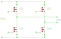
\includegraphics[width = 3.5in]{hBridge}
\caption{The H-bridge circuit showing switching-leg pairs (Q1, Q2) and (Q3, Q4)}, and opposing-leg pairs (Q1, Q4) and (Q2, Q3)
\label{hBridge}
\end{figure}


\subsection{Bipolar PWM}
The operation of a bipolar switching scheme generally operates as follows:
\begin{equation}
\begin{cases}
\label{bipolarStates}
V_{out} = V_{dc} &\mbox{if $V_{ref} > V_{c}$} \\
V_{out} = -V_{dc} &\mbox{if $V_{ref} < V_{c}$}
\end{cases}
\end{equation}

In this inversion scheme, opposing switching pairs are modulated simulataneously. 
Where $V_{ref}$ is the reference signal, and $V_c$ is the carrier signal. In Figure \ref{bipolarSwitchingOperation} we can see that $V_{out} = V_{AO}-V_{BO}$ resulting in an output that exists only in one of the two states described in equation \ref{bipolarStates}. If we select an odd modulation index, the output waveform exhibits odd-symetry and we can effectively eliminate all even harmonics at the output.

\begin{figure}
\centering
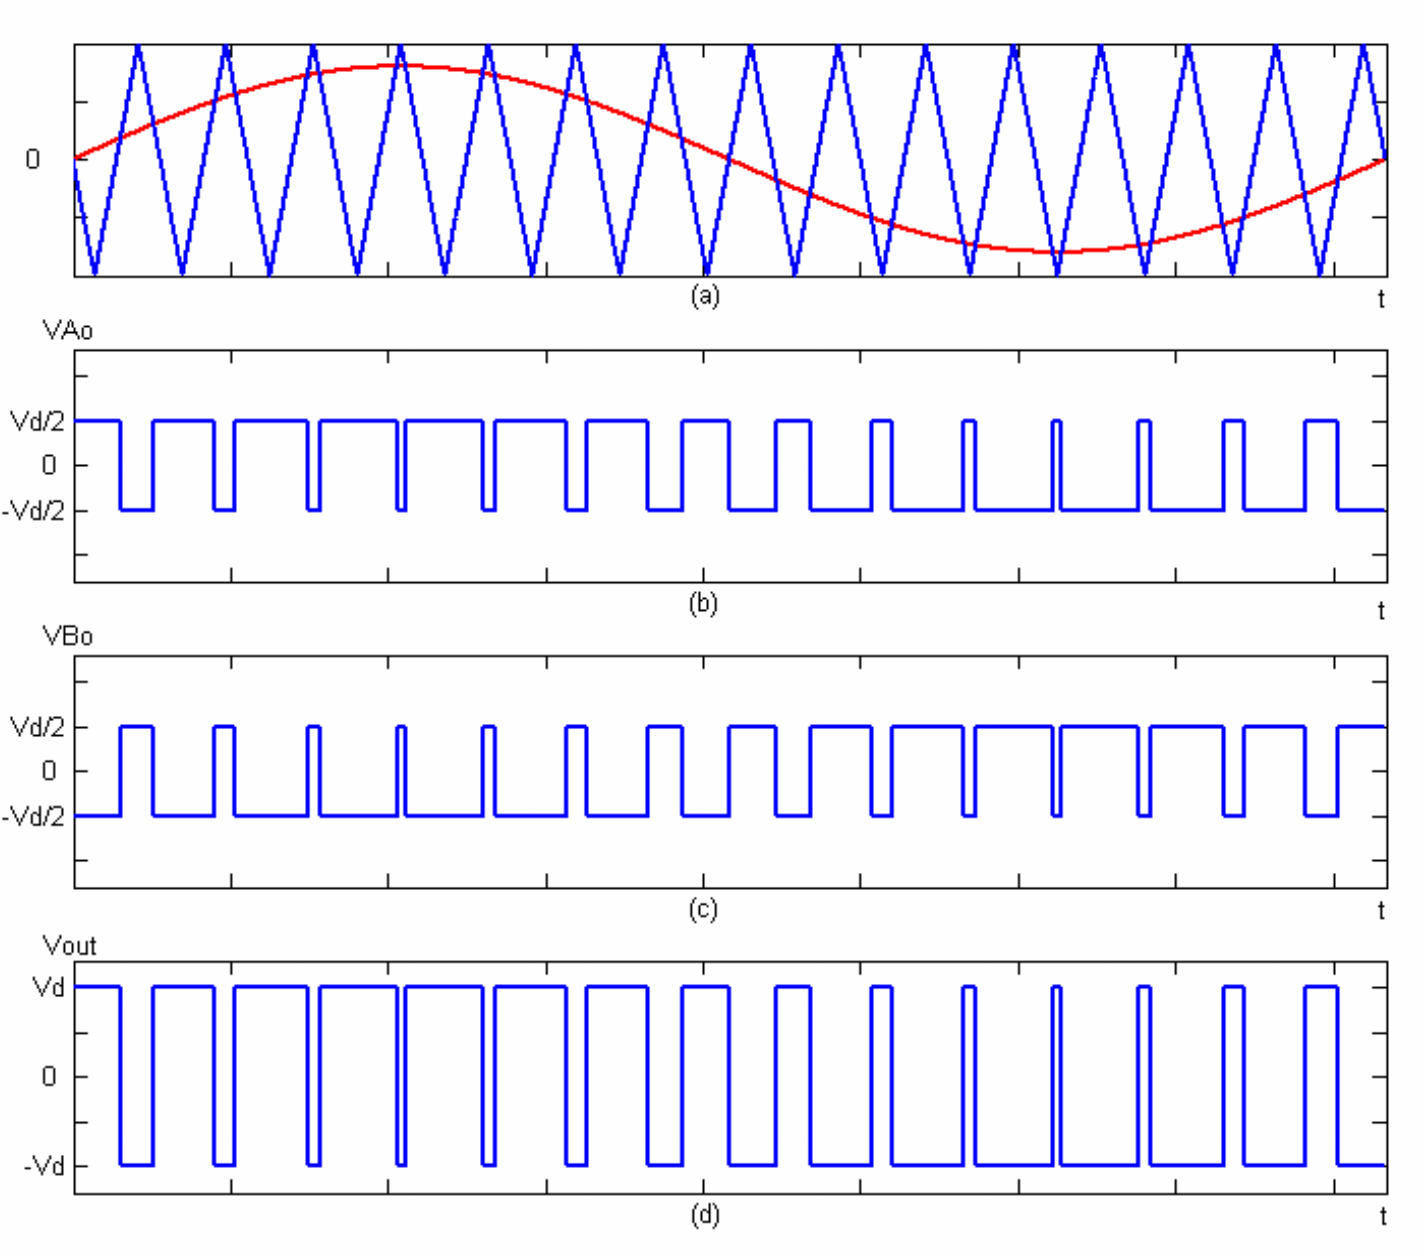
\includegraphics[width = 3.5in]{bipolarPwmShot}
\caption{The operation of a bipolar switching scheme for an inverter.\cite{fourierAnalysis}} 
\label{bipolarSwitchingOperation}
\end{figure}

\subsection{Unipolar PWM}
The operation of the unipolar PWM works under the following rules, given a triangular carrier signal and a sinusoidal reference. Note that in Figure \ref{unipolarStates}, ${V_{control}}_{1}$

\begin{equation}
\label{unipolarStates}
\begin{cases}
V_{out} = V_{dc} &\mbox{if $V_{ref} > V_{c}$}  \\
V_{out} = -V_{dc} &\mbox{if $V_{ref} < V_{c}$}  \\
V_{out} = 0 &\mbox{if $V_{ref} < V_{c}$}  \\
\end{cases}
\end{equation}



\begin{figure}
\centering
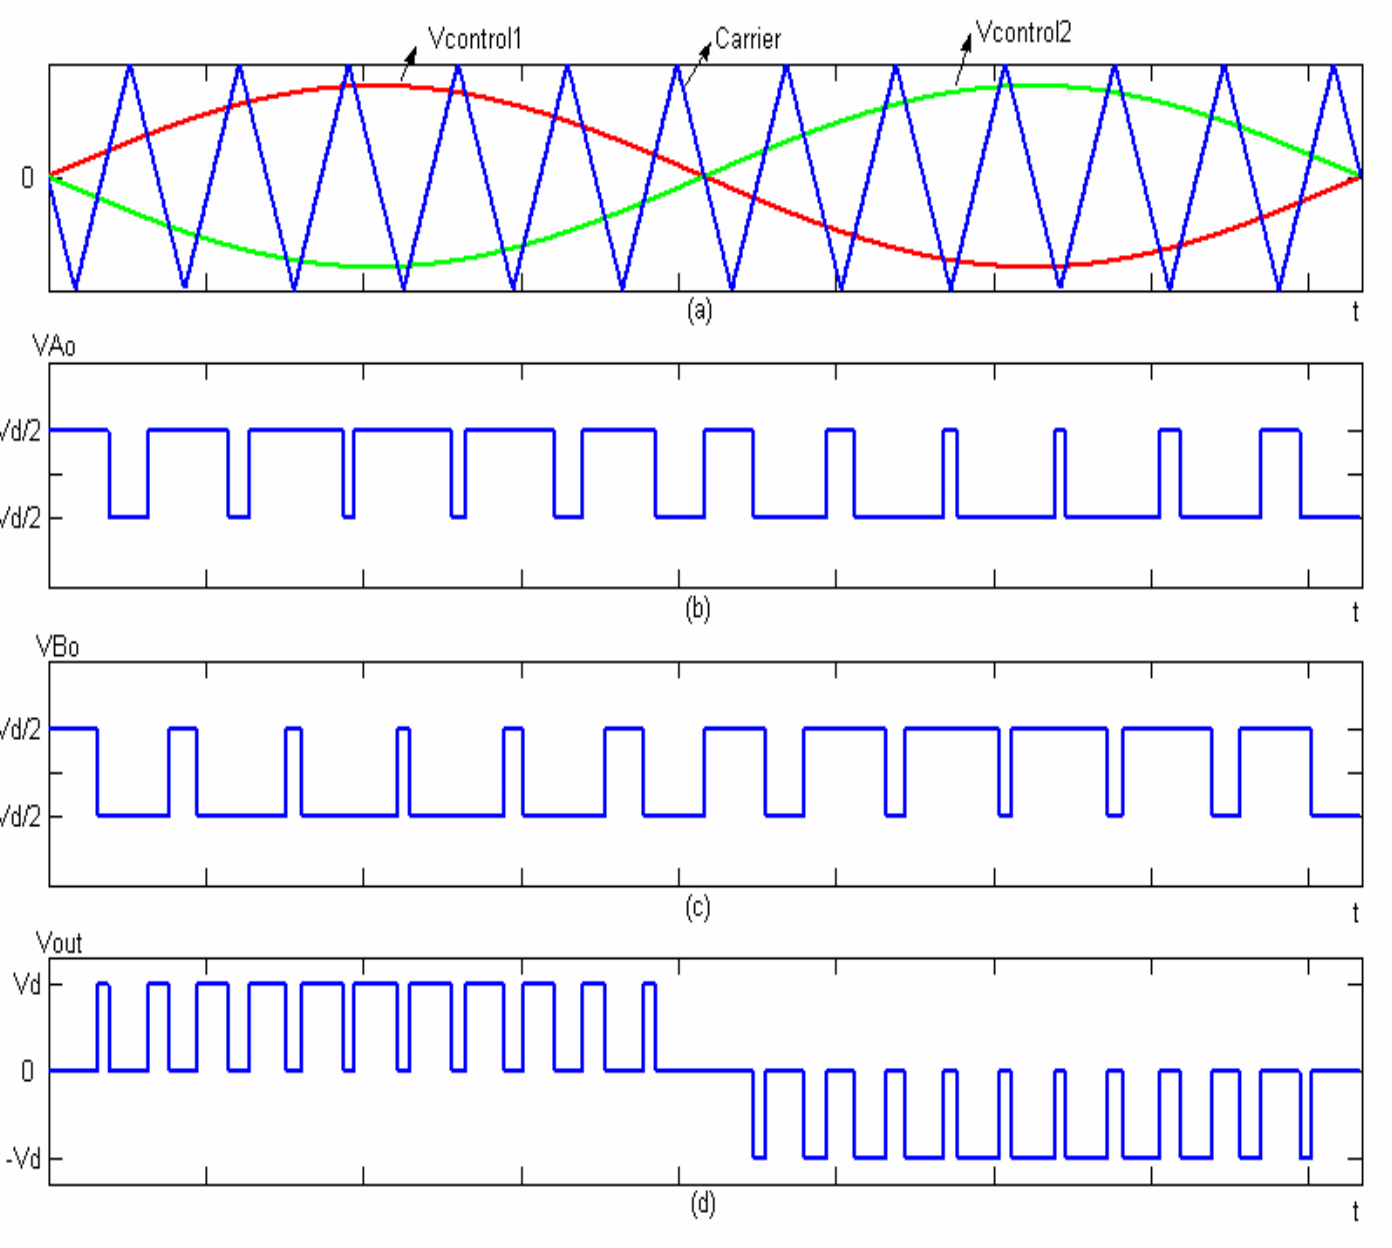
\includegraphics[width = 3.5in]{unipolarPwmShot}
\caption{The operation of a unipolar switching scheme for an inverter. Note that a single control signal is used in our software implementation since each control signal is the other's dual. \cite{fourierAnalysis}}
\label{unipolarPwmShot}
\end{figure}

\subsection{Hybrid PWM}

\section{PWM Performance}
In this section we undertake a comparative study of the three PWM techniques that have been the focus of much of this work: bipolar and unipolar PWM, and the hybrid PWM. We have taken our results mainly from two sources aside from the purely mathematical results obtained for bipolar and unipolar PWM given above. First, we compare state the results of fourier analysis in Matlab/Simulink using the fast fourier transform (FFT). Next, we discuss how the unipolar and hybrid PWM techniques fair in our real-world tests on the hybrid inverter team development board. These reults are obtained using the FFT functionality of a Techtroniks oscilloscope. \todo[inline]{get full scope name} 
\subsection{Bipolar PWM}
In Simulink we implemented a simple bipolar inverter and performed an FFT using the powerGUI in SimPower Systems. The results are shown in Figure \ref{bipolarFFTMatlab}. The THD of this signal is found to be nearly $147\%$, and we note that the harmonics at the the frequency of modulation are greater than the funamentals for this scheme.

\begin{figure}
\centering
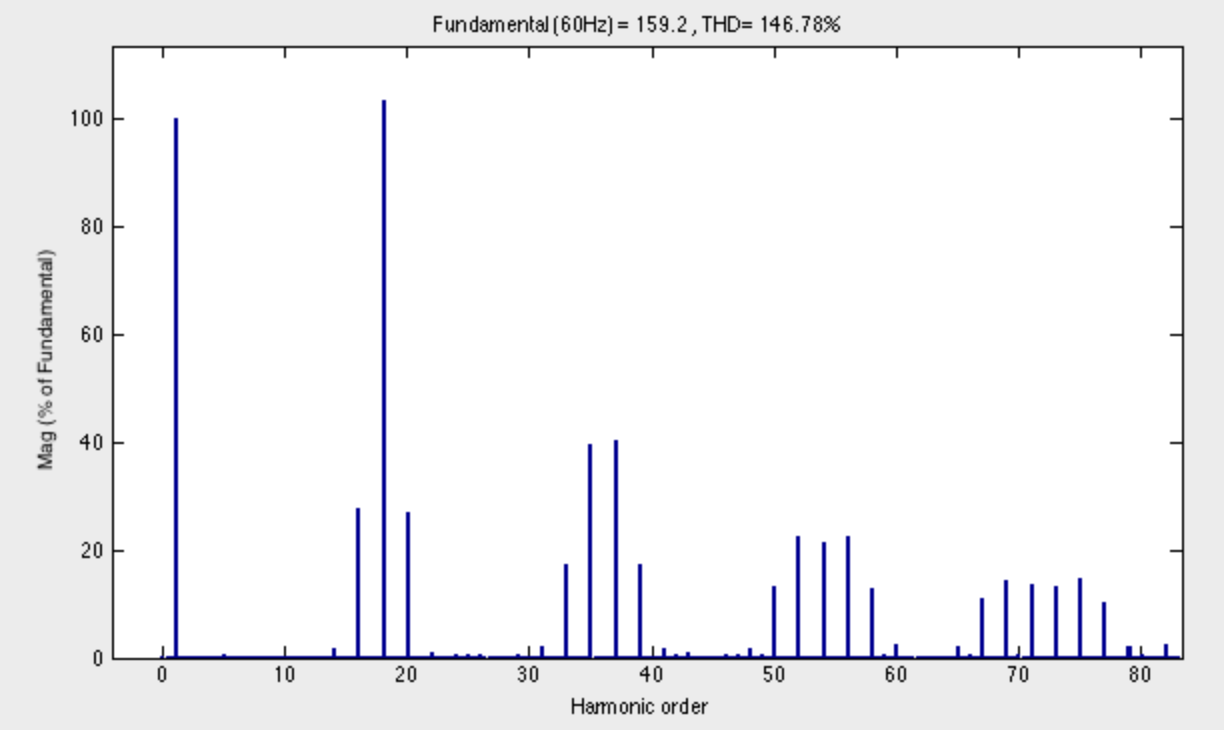
\includegraphics[width = 3.5in]{bipolarFFTMatlab}
\caption{The spectral content of a bipolar inverter is given by FFT, with harmonics shown as multiples of the fundamental at 60Hz}
\label{bipolarFFTMatlab}
\end{figure}
\todo[inline]{include fourier analysis equations from 13}

Due to time constraints, we were not able to perform analyses on a bipolar inverter in hardware; the focus of this work is on the industry standard unipolar scheme discussed in the next subsection. 
\subsection{Unipolar PWM}

Again, using Simulink we implemented a unipolar inverter and performed an FFT using the powerGUI in SimPower Systems. The results are shown in Figure \ref{unipolarFFTMatlab}. The THD of this signal is found to be around $77\%$, or nearly half that of the bipolar scheme. Here, the magnitdude of the fundamental is greater than any of the harmonics. These results confirm those of \cite{fourierAnalysis}, though we found the THD of the bipolar scheme in our simulation to be much higher. Both measurements were taken before any kind of filtering stage. 

\begin{figure}
\centering
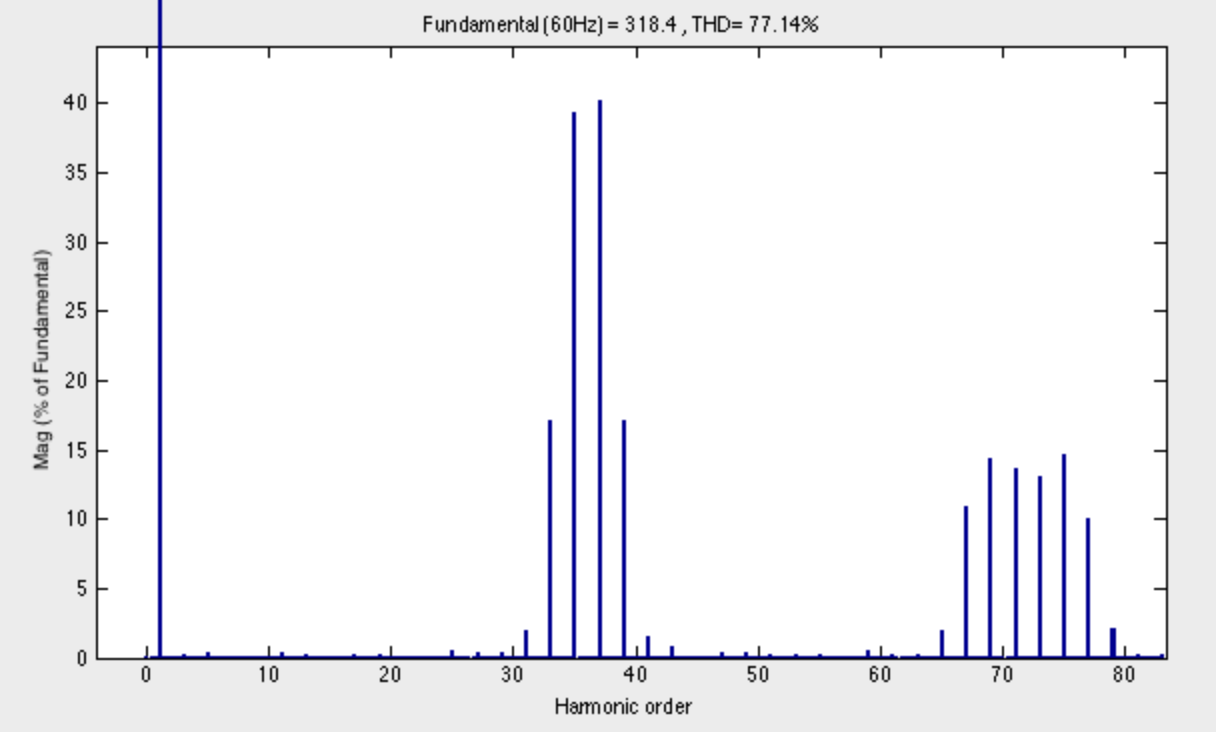
\includegraphics[width = 3.5in]{unipolarFFTMatlab}
\caption{The spectral content of a unipolar inverter is given by FFT, with harmonics shown as multiples of the fundamental at 60Hz}
\label{unipolarFFTMatlab}
\end{figure}

\todo[inline]{include fourier analysis from 13}


\section{Hybrid Performance}

\section{Conclusion}
